\subsection{Full-budget model-envelope refinement and every primary SCIP mask}\label{app:refined-external-v91}
All twenty primary masks receive the same-objective SCIP control. The four existing first-mask runs are reused and sixteen additional runs use unchanged candidates, boxes, regularization and initial midpoint witnesses. A ten-second nominal complete budget and $10^{-10}$ search tolerance match the primary search. All seed-level endpoints and actual costs are supplied.

ZORRO's valid unsplit fixed point is also retained as a parent bound. Within the same complete ten-second cap, a best-first queue refines the box with the largest upper. Its regret-polynomial coefficient sensitivities select a split coordinate once a model envelope exists; the fixed-point existence stage uses its geometric coordinate score. Both children inherit their legal parent's upper immediately. A completed child envelope can tighten that bound; incomplete work leaves the inherited upper available. All data/model shared symbols and the original $\lambda$ remain in the conversion. Original-table midpoint fits update feasible lowers. This gives a valid complete cover at every time, including partial refinement. The original single-envelope results remain in Table~\ref{tab:zorro-v90}.

\begin{table*}[t]\centering\small
\caption{Full-budget ZORRO refinement on the same four first-mask instances. Widths use $10^{-6}$ units. Every attempted call enters actual complete cost; the plot credits completed evidence by its timestamp.}
\label{tab:zorro-refined-v91}
\begin{tabular}{lrrrrr}\toprule Data&Single-envelope width&Refined width&Completed envelopes&Complete seconds&Model-envelope cover\\\midrule
Supercond. & 185.998 & 185.998 & 0 & 10.058 & --\\
Parkinsons & 17.134 & 10.063 & 15 & 10.047 & yes\\
Wine Quality & 4.503 & 3.200 & 24 & 10.339 & yes\\
Yacht & 19.788 & 2.014 & 41 & 10.183 & yes\\
\bottomrule\end{tabular}\end{table*}
The independent rational audit checks all eighty model-envelope bounds used by refinement on the three completed-model tasks, each shared-symbol regret conversion, every parent-bound inheritance, and complete binary partition coverage. Superconductivity retains the previously checked common cap. Figure~\ref{fig:zorro-time-v91} compares completed-width trajectories, including each method's full setup and candidate/input cost.
\begin{figure*}[t]\centering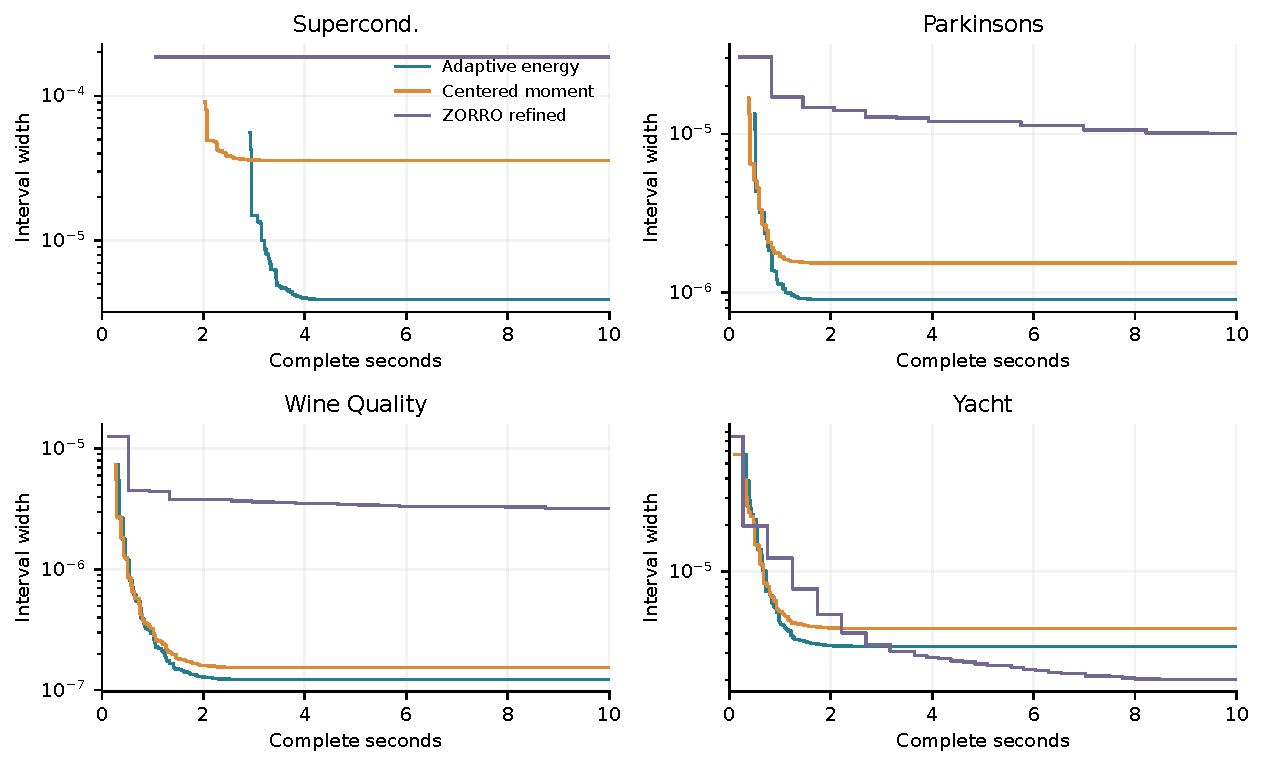
\includegraphics[width=.97\textwidth]{images/zorro_refinement_v91.pdf}
\caption{Same-instance width against complete computation time. A and M keep their numerical/tail-floor endpoints once finished. Refined ZORRO preserves the parent's valid upper during incomplete child work and uses the full cap. All widths are in normalized objective units.}
\label{fig:zorro-time-v91}\end{figure*}
